%%%%%%%%%%%%%%%%%%%%%%%%%%%%%%%%%%%%%%%%%%%%%%%%%%%%%%%%%%%%%%%%%%%%%%%
%% Reviews of Accelerator Science and Technology
%% Trim Size: 11in x 8.5in
%% Text Area: 9.25in (include runningheads) x 6.6in
%% Main Text: 10/13pt
%% Date:      16-04-2014
%%%%%%%%%%%%%%%%%%%%%%%%%%%%%%%%%%%%%%%%%%%%%%%%%%%%%%%%%%%%%%%%%%%%%%%

%\documentclass[wsdraft]{ws-rast} % to draw visible frames for the text
%\documentclass[twocolumn]{ws-rast}
\documentclass[]{report}
\usepackage{amsmath}
\usepackage{amssymb}
\usepackage{graphicx}
\usepackage{url}
\usepackage{hyperref}

\usepackage[displaymath]{lineno}


\usepackage{bm}
\usepackage{amsmath}
\usepackage{amssymb}
\usepackage{graphicx}
\usepackage{url}
\usepackage{hyperref}

\usepackage[displaymath]{lineno}\usepackage{bm}% bold math

\newcommand{\fe}{\mathbf{\tilde{E}}}
\newcommand{\fb}{\mathbf{\tilde{B}}}
\newcommand{\fj}{\mathbf{\tilde{J}}}
\newcommand{\ff}{\tilde{F}}
\newcommand{\fg}{\tilde{G}}
\newcommand{\fk}{\mathbf{k}}
\newcommand{\fkhat}{\mathbf{\hat{k}}}

% Definitions from Remi's paper on Galilean math
\newcommand{\Km}{\vec{K}_{\vec{m}}}
\newcommand{\km}{\vec{k}_{\vec{m}}}
\renewcommand{\vec}[1]{\boldsymbol{#1}}
\newcommand{\vgal}{\vec{v}_{gal}}
\newcommand{\nab}{\vec{\nabla'}}
\newcommand{\Dt}[1]{ \frac{\partial #1}{\partial t}}
\newcommand{\mc}[1]{\hat{\mathcal{#1}}}
\newcommand{\xj}{\vec{x}'_{\vec{j}}}
\newcommand{\Xll}{\vec{X}_{\vec{\ell}}}
\newcommand{\Integ}[1]{\int_{-\infty}^{\infty} \!\!\!\!\!\!
  \mathrm{d}#1}
\newcommand{\RInteg}[1]{\int_{0}^{\infty} \!\! \frac{#1\mathrm{d}#1}{(2\pi)^2}}

% Definitions from Remi's Thesis
\newcommand{\h}{\mathcal{H}}
\newcommand{\hf}{\frac{1}{2}}
\newcommand{\um}{$\mu$m}
\newcommand{\Um}{\mu \mathrm{m}}
\newcommand{\aal}{\langle \vec{a}_l^2 \rangle}
\newcommand{\etad}{ \eta_d }
\newcommand{\etae}{ \eta_\epsilon }
\newcommand{\etag}{ \eta_\gamma }
\newcommand{\tlambda}{ \tilde{\lambda} }
%\newcommand\comment[1]{\textcolor{red}{\textbf{#1}}}
\newcommand{\gsim}{\mathrel{\hbox{\rlap{\lower.55ex 
\hbox{$\sim$}} \kern-.3em \raise.4ex \hbox{$>$}}}}
\newcommand{\lsim}{\mathrel{\hbox{\rlap{\lower.55ex 
\hbox{$\sim$}} \kern-.3em \raise.4ex \hbox{$<$}}}}
\newcommand{\kfoc}{k_\mathrm{foc}}
\newcommand{\bkfoc}{\bar{k}_\mathrm{foc}}
\newcommand{\xil}{\xi_{\mathrm{laser}}}

\newcommand{\Ex}[2]{{E_x}^{#1}_{#2}}
\newcommand{\Ey}[2]{{E_y}^{#1}_{#2}}
\newcommand{\Ez}[2]{{E_z}^{#1}_{#2}}
\newcommand{\Bx}[2]{{B_x}^{#1}_{#2}}
\newcommand{\By}[2]{{B_y}^{#1}_{#2}}
\newcommand{\Bz}[2]{{B_z}^{#1}_{#2}}
\newcommand{\Jx}[2]{{J_x}^{#1}_{#2}}
\newcommand{\Jy}[2]{{J_y}^{#1}_{#2}}
\newcommand{\Jz}[2]{{J_z}^{#1}_{#2}}

\newcommand{\tEr}[2]{\tilde{E_r}^{#1}_{#2}}
\newcommand{\tEt}[2]{\tilde{E_\theta}^{#1}_{#2}}
\newcommand{\tEz}[2]{\tilde{E_z}^{#1}_{#2}}
\newcommand{\tBr}[2]{\tilde{B_r}^{#1}_{#2}}
\newcommand{\tBt}[2]{\tilde{B_\theta}^{#1}_{#2}}
\newcommand{\tBz}[2]{\tilde{B_z}^{#1}_{#2}}
\newcommand{\tJr}[2]{\tilde{J_r}^{#1}_{#2}}
\newcommand{\tJt}[2]{\tilde{J_\theta}^{#1}_{#2}}
\newcommand{\tJz}[2]{\tilde{J_z}^{#1}_{#2}}

\newcommand{\CCirc}{\textsc{Calder Circ}}
\newcommand{\CCart}{\textsc{Calder 3D}}

\begin{document}

\markboth{J.-L. Vay, R. Lehe}{Simulations for plasma and laser acceleration.}

\title{WarpX}

%\author{Jean-Luc Vay, R\'emi Lehe}
%\address{Lawrence Berkeley National Laboratory, Berkeley, California, USA\\
%\email{jlvay@lbl.gov}}

%\address{Lawrence Berkeley National Laboratory, Berkeley, California, USA\\
%\email{rlehe@lbl.gov}}

\maketitle

\linenumbers

\begin{abstract}
Computer simulations have had a profound impact on the design and understanding of past and present plasma acceleration experiments, and will be a key component for turning plasma accelerators from a promising technology into a mainstream scientific tool. In this chapter, we present an overview of the numerical techniques used with the most popular approaches to model plasma-based accelerators: electromagnetic Particle-In-Cell, Quasi-Static, Ponderomotive Guiding Center.
The material that is presented is intended to serve as an introduction to the basics of those approaches, and to advances (some of them very recent) that have pushed the state-of-the-art, such as optimal Lorentz boosted frame, advanced laser envelope solvers and the elimination of numerical Cherenkov instability. The Particle-In-Cell method, which has broader interest and is more standardized, is presented in more depth. Additional topics that are cross-cutting such as azimuthal Fourier decomposition or filtering are also discussed, as well as potential challenges and remedies in the initialization of simulations and output of data.  Examples of simulations using the techniques that are presented have been left out of this chapter for conciseness, and because simulation results are best understood when presented together - and contrasted with - theoretical and/or experimental results, as in other chapters of this volume.
\end{abstract}

%%%%%%%%%%%%%%%%%%%%%%%%%%%%%%%%%%%
\section{Introduction}
%%%%%%%%%%%%%%%%%%%%%%%%%%%%%%%%%%%

\begin{figure}
%\begin{centering}
%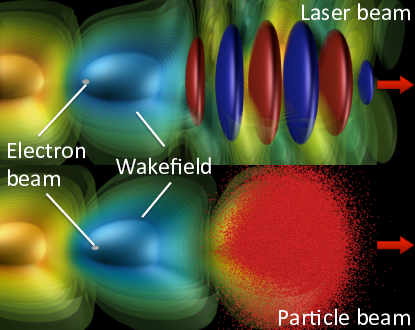
\includegraphics[trim={6cm 4cm 5cm 5cm},clip,scale=0.5]{Plasma_acceleration_sim.pdf}
%\immediate\write18{curl http://hifweb.lbl.gov/public/WarpX/test.png > Plasma_acceleration_sim.png}
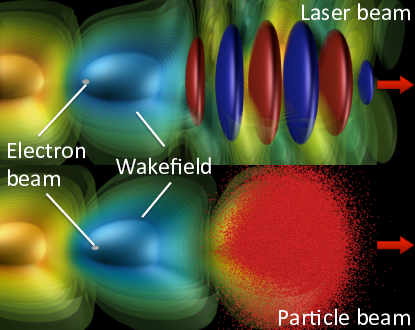
\includegraphics[scale=0.5]{Plasma_acceleration_sim.png}

%\par\end{centering}
\caption{\label{fig:Plasma_acceleration_sim} Plasma laser-driven (top) and charged-particles-driven (bottom) acceleration (rendering from 3-D Particle-In-Cell simulations). A laser beam (red and blue disks in top picture) or a charged particle beam (red dots in bottom picture) propagating (from left to right) through an under-dense plasma (not represented) displaces electrons, creating a plasma wakefield that supports very high electric fields (pale blue and yellow). These electric fields, which can be orders of magnitude larger than with conventional techniques, can be used to accelerate a short charged particle beam (white) to high-energy over a very short distance.}
\end{figure}

Computer simulations have had a profound impact on the design and understanding of past and present plasma acceleration experiments \cite{Tsungpop06,Geddesjp08,Geddesscidac09,Huangscidac09}, with
accurate modeling of wake formation, electron self-trapping and acceleration requiring fully kinetic methods (usually Particle-In-Cell) using large computational resources due to the wide range of space and time scales involved. Numerical modeling complements and guides the design and analysis of advanced accelerators, and can reduce development costs significantly. Despite the major recent experimental successes\cite{LeemansPRL2014,Blumenfeld2007,BulanovSV2014,Steinke2016}, the various advanced acceleration concepts need significant progress to fulfill their potential.  To this end, large-scale simulations will continue to be a key component toward reaching a detailed understanding of the complex interrelated physics phenomena at play.

For such simulations,
the most popular algorithm is the Particle-In-Cell (or PIC) technique,
which represents electromagnetic fields on a grid and particles by
a sample of macroparticles.
However, these simulations are extremely computationally intensive, due to the need to resolve the evolution of a driver (laser or particle beam) and an accelerated beam into a structure that is orders of magnitude longer and wider than the accelerated beam.
Various techniques or reduced models have been developed to allow multidimensional simulations at manageable computational costs: quasistatic approximation \cite{Sprangleprl90,Antonsenprl1992,Krallpre1993,Morapop1997,Quickpic},
ponderomotive guiding center (PGC) models \cite{Antonsenprl1992,Krallpre1993,Quickpic,Benedettiaac2010,Cowanjcp11}, simulation in an optimal Lorentz boosted frame \cite{Vayprl07,Bruhwileraac08,Vayscidac09,Vaypac09,Martinspac09,VayAAC2010,Martinsnaturephysics10,Martinspop10, Martinscpc10, Vayjcp2011,VayPOPL2011,Vaypop2011,Yu2016},
expanding the fields into a truncated series of azimuthal modes
\cite{godfrey1985iprop,LifschitzJCP2009,DavidsonJCP2015,Lehe2016,AndriyashPoP2016}, fluid approximation \cite{Krallpre1993,Shadwickpop09,Benedettiaac2010} and scaled parameters \cite{Cormieraac08,Geddespac09}.
%
Many codes have been developed and are used for the modeling of plasma accelerators.
A list of such codes is given in table \ref{table_codes}, with the name of the code, its main characteristics, the web site if existing or a reference, and the availability and license, if known.

In Section 2 of this chapter, we review the standard methods employed in relativistic electromagnetic Particle-In-Cell (PIC) simulations of plasma accelerators, including the core PIC loop steps (particle push, fields update, current deposition from the particles to the grid and fields gathering from the grid to the particles positions), the use of moving window and Lorentz boosted frame, the numerical Cherenkov instability and its mitigation. The electromagnetic quasistatic approximation is presented in section 3, the ponderomotive guiding center approximation in section 4, and azimuthal Fourier decomposition in section 5. Additional considerations such as filtering and inputs/outputs are discussed respectively in sections 6 and 7.

%%%%%%%%%%%%%%%%%%%%%%%%%%%%%%%%%%%
\section{The electromagnetic Particle-In-Cell method}
%%%%%%%%%%%%%%%%%%%%%%%%%%%%%%%%%%%

\begin{figure}
%\begin{centering}
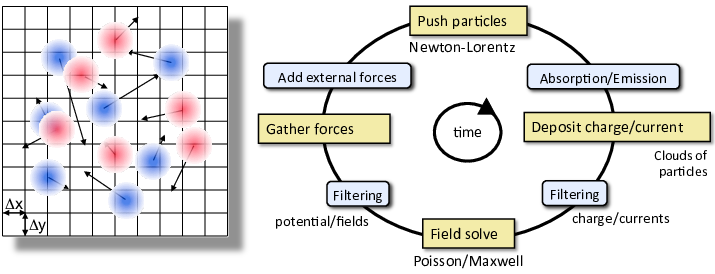
\includegraphics[scale=0.6]{PIC.png}
%\par\end{centering}
\caption{\label{fig:PIC} The Particle-In-Cell (PIC) method follows the evolution of a collection of charged macro-particles (positively charged in blue on the left plot, negatively charged in red) that evolve self-consistently with their electromagnetic (or electrostatic) fields. The core PIC algorithm involves four operations at each time step: 1) evolve the velocity and position of the particles using the Newton-Lorentz equations, 2) deposit the charge and/or current densities through interpolation from the particles distributions onto the grid, 3) evolve Maxwell's wave equations (for electromagnetic) or solve Poisson's equation (for electrostatic) on the grid, 4) interpolate the fields from the grid onto the particles for the next particle push. Additional ``add-ons'' operations are inserted between these core operations to account for additional physics (e.g. absorption/emission of particles, addition of external forces to account for accelerator focusing or accelerating component) or numerical effects (e.g. smoothing/filtering of the charge/current densities and/or fields on the grid).}
\end{figure}

In the electromagnetic Particle-In-Cell method \cite{Birdsalllangdon},
the electromagnetic fields are solved on a grid, usually using Maxwell's
equations

\begin{subequations}
\begin{eqnarray}
\frac{\mathbf{\partial B}}{\partial t} & = & -\nabla\times\mathbf{E}\label{Eq:Faraday-1}\\
\frac{\mathbf{\partial E}}{\partial t} & = & \nabla\times\mathbf{B}-\mathbf{J}\label{Eq:Ampere-1}\\
\nabla\cdot\mathbf{E} & = & \rho\label{Eq:Gauss-1}\\
\nabla\cdot\mathbf{B} & = & 0\label{Eq:divb-1}
\end{eqnarray}
\end{subequations}
given here in natural units ($\epsilon_0=\mu_0=c=1$), where $t$ is time, $\mathbf{E}$ and
$\mathbf{B}$ are the electric and magnetic field components, and
$\rho$ and $\mathbf{J}$ are the charge and current densities. The
charged particles are advanced in time using the Newton-Lorentz equations
of motion
\begin{subequations}
\begin{align}
\frac{d\mathbf{x}}{dt}= & \mathbf{v},\label{Eq:Lorentz_x-1}\\
\frac{d\left(\gamma\mathbf{v}\right)}{dt}= & \frac{q}{m}\left(\mathbf{E}+\mathbf{v}\times\mathbf{B}\right),\label{Eq:Lorentz_v-1}
\end{align}
\end{subequations}
where $m$, $q$, $\mathbf{x}$, $\mathbf{v}$ and $\gamma=1/\sqrt{1-v^{2}}$
 are respectively the mass, charge, position, velocity and relativistic
factor of the particle given in natural units ($c=1$). The charge and current densities are interpolated
on the grid from the particles' positions and velocities, while the
electric and magnetic field components are interpolated from the grid
to the particles' positions for the velocity update.

%%%%%%%%%%%%%%%%%%%%%%%%%%%%%%%%%%%
\subsection{Particle push}
%%%%%%%%%%%%%%%%%%%%%%%%%%%%%%%%%%%

A centered finite-difference discretization of the Newton-Lorentz
equations of motion is given by
\begin{subequations}
\begin{align}
\frac{\mathbf{x}^{i+1}-\mathbf{x}^{i}}{\Delta t}= & \mathbf{v}^{i+1/2},\label{Eq:leapfrog_x}\\
\frac{\gamma^{i+1/2}\mathbf{v}^{i+1/2}-\gamma^{i-1/2}\mathbf{v}^{i-1/2}}{\Delta t}= & \frac{q}{m}\left(\mathbf{E}^{i}+\mathbf{\bar{v}}^{i}\times\mathbf{B}^{i}\right).\label{Eq:leapfrog_v}
\end{align}
\end{subequations}
In order to close the system, $\bar{\mathbf{v}}^{i}$ must be
expressed as a function of the other quantities. The two implementations that have become the most popular are presented below.

%%%%%%%%%%%%%%%%%%%%%%%%%%%%%%%%%%%
\subsubsection{Boris relativistic velocity rotation}
%%%%%%%%%%%%%%%%%%%%%%%%%%%%%%%%%%%

\usepackage{bm}
\usepackage{amsmath}
\usepackage{amssymb}
\usepackage{graphicx}
\usepackage{url}
\usepackage{hyperref}

\usepackage[displaymath]{lineno}\usepackage{bm}% bold math

\newcommand{\fe}{\mathbf{\tilde{E}}}
\newcommand{\fb}{\mathbf{\tilde{B}}}
\newcommand{\fj}{\mathbf{\tilde{J}}}
\newcommand{\ff}{\tilde{F}}
\newcommand{\fg}{\tilde{G}}
\newcommand{\fk}{\mathbf{k}}
\newcommand{\fkhat}{\mathbf{\hat{k}}}

% Definitions from Remi's paper on Galilean math
\newcommand{\Km}{\vec{K}_{\vec{m}}}
\newcommand{\km}{\vec{k}_{\vec{m}}}
\renewcommand{\vec}[1]{\boldsymbol{#1}}
\newcommand{\vgal}{\vec{v}_{gal}}
\newcommand{\nab}{\vec{\nabla'}}
\newcommand{\Dt}[1]{ \frac{\partial #1}{\partial t}}
\newcommand{\mc}[1]{\hat{\mathcal{#1}}}
\newcommand{\xj}{\vec{x}'_{\vec{j}}}
\newcommand{\Xll}{\vec{X}_{\vec{\ell}}}
\newcommand{\Integ}[1]{\int_{-\infty}^{\infty} \!\!\!\!\!\!
  \mathrm{d}#1}
\newcommand{\RInteg}[1]{\int_{0}^{\infty} \!\! \frac{#1\mathrm{d}#1}{(2\pi)^2}}

% Definitions from Remi's Thesis
\newcommand{\h}{\mathcal{H}}
\newcommand{\hf}{\frac{1}{2}}
\newcommand{\um}{$\mu$m}
\newcommand{\Um}{\mu \mathrm{m}}
\newcommand{\aal}{\langle \vec{a}_l^2 \rangle}
\newcommand{\etad}{ \eta_d }
\newcommand{\etae}{ \eta_\epsilon }
\newcommand{\etag}{ \eta_\gamma }
\newcommand{\tlambda}{ \tilde{\lambda} }
%\newcommand\comment[1]{\textcolor{red}{\textbf{#1}}}
\newcommand{\gsim}{\mathrel{\hbox{\rlap{\lower.55ex 
\hbox{$\sim$}} \kern-.3em \raise.4ex \hbox{$>$}}}}
\newcommand{\lsim}{\mathrel{\hbox{\rlap{\lower.55ex 
\hbox{$\sim$}} \kern-.3em \raise.4ex \hbox{$<$}}}}
\newcommand{\kfoc}{k_\mathrm{foc}}
\newcommand{\bkfoc}{\bar{k}_\mathrm{foc}}
\newcommand{\xil}{\xi_{\mathrm{laser}}}

\newcommand{\Ex}[2]{{E_x}^{#1}_{#2}}
\newcommand{\Ey}[2]{{E_y}^{#1}_{#2}}
\newcommand{\Ez}[2]{{E_z}^{#1}_{#2}}
\newcommand{\Bx}[2]{{B_x}^{#1}_{#2}}
\newcommand{\By}[2]{{B_y}^{#1}_{#2}}
\newcommand{\Bz}[2]{{B_z}^{#1}_{#2}}
\newcommand{\Jx}[2]{{J_x}^{#1}_{#2}}
\newcommand{\Jy}[2]{{J_y}^{#1}_{#2}}
\newcommand{\Jz}[2]{{J_z}^{#1}_{#2}}

\newcommand{\tEr}[2]{\tilde{E_r}^{#1}_{#2}}
\newcommand{\tEt}[2]{\tilde{E_\theta}^{#1}_{#2}}
\newcommand{\tEz}[2]{\tilde{E_z}^{#1}_{#2}}
\newcommand{\tBr}[2]{\tilde{B_r}^{#1}_{#2}}
\newcommand{\tBt}[2]{\tilde{B_\theta}^{#1}_{#2}}
\newcommand{\tBz}[2]{\tilde{B_z}^{#1}_{#2}}
\newcommand{\tJr}[2]{\tilde{J_r}^{#1}_{#2}}
\newcommand{\tJt}[2]{\tilde{J_\theta}^{#1}_{#2}}
\newcommand{\tJz}[2]{\tilde{J_z}^{#1}_{#2}}

\newcommand{\CCirc}{\textsc{Calder Circ}}
\newcommand{\CCart}{\textsc{Calder 3D}}

The solution proposed by Boris \cite{BorisICNSP70} is given by 
\begin{align}
\mathbf{\bar{v}}^{i}= & \frac{\gamma^{i+1/2}\mathbf{v}^{i+1/2}+\gamma^{i-1/2}\mathbf{v}^{i-1/2}}{2\bar{\gamma}^{i}}.\label{Eq:boris_v}
\end{align}
where $\bar{\gamma}^{i}$ is defined by $\bar{\gamma}^{i} \equiv (\gamma^{i+1/2}+\gamma^{i-1/2} )/2$.

The system (\ref{Eq:leapfrog_v},\ref{Eq:boris_v}) is solved very
efficiently following Boris' method, where the electric field push
is decoupled from the magnetic push. Setting $\mathbf{u}=\gamma\mathbf{v}$, the
velocity is updated using the following sequence:

\begin{subequations}
\begin{align}
\mathbf{u^{-}}= & \mathbf{u}^{i-1/2}+\left(q\Delta t/2m\right)\mathbf{E}^{i}\\
\mathbf{u'}= & \mathbf{u}^{-}+\mathbf{u}^{-}\times\mathbf{t}\\
\mathbf{u}^{+}= & \mathbf{u}^{-}+\mathbf{u'}\times2\mathbf{t}/(1+t^{2})\\
\mathbf{u}^{i+1/2}= & \mathbf{u}^{+}+\left(q\Delta t/2m\right)\mathbf{E}^{i}
\end{align}
\end{subequations}
where $\mathbf{t}=\left(q\Delta
  t/2m\right)\mathbf{B}^{i}/\bar{\gamma}^{i}$ and where
$\bar{\gamma}^{i}$ can be calculated as $\bar{\gamma}^{i}=\sqrt{1+(\mathbf{u}^-/c)^2}$. 

The Boris implementation is second-order accurate, time-reversible and fast. Its implementation is very widespread and used in the vast majority of PIC codes.


%%%%%%%%%%%%%%%%%%%%%%%%%%%%%%%%%%%
\subsubsection{Vay Lorentz-invariant formulation}
%%%%%%%%%%%%%%%%%%%%%%%%%%%%%%%%%%%

\usepackage{bm}
\usepackage{amsmath}
\usepackage{amssymb}
\usepackage{graphicx}
\usepackage{url}
\usepackage{hyperref}

\usepackage[displaymath]{lineno}\usepackage{bm}% bold math

\newcommand{\fe}{\mathbf{\tilde{E}}}
\newcommand{\fb}{\mathbf{\tilde{B}}}
\newcommand{\fj}{\mathbf{\tilde{J}}}
\newcommand{\ff}{\tilde{F}}
\newcommand{\fg}{\tilde{G}}
\newcommand{\fk}{\mathbf{k}}
\newcommand{\fkhat}{\mathbf{\hat{k}}}

% Definitions from Remi's paper on Galilean math
\newcommand{\Km}{\vec{K}_{\vec{m}}}
\newcommand{\km}{\vec{k}_{\vec{m}}}
\renewcommand{\vec}[1]{\boldsymbol{#1}}
\newcommand{\vgal}{\vec{v}_{gal}}
\newcommand{\nab}{\vec{\nabla'}}
\newcommand{\Dt}[1]{ \frac{\partial #1}{\partial t}}
\newcommand{\mc}[1]{\hat{\mathcal{#1}}}
\newcommand{\xj}{\vec{x}'_{\vec{j}}}
\newcommand{\Xll}{\vec{X}_{\vec{\ell}}}
\newcommand{\Integ}[1]{\int_{-\infty}^{\infty} \!\!\!\!\!\!
  \mathrm{d}#1}
\newcommand{\RInteg}[1]{\int_{0}^{\infty} \!\! \frac{#1\mathrm{d}#1}{(2\pi)^2}}

% Definitions from Remi's Thesis
\newcommand{\h}{\mathcal{H}}
\newcommand{\hf}{\frac{1}{2}}
\newcommand{\um}{$\mu$m}
\newcommand{\Um}{\mu \mathrm{m}}
\newcommand{\aal}{\langle \vec{a}_l^2 \rangle}
\newcommand{\etad}{ \eta_d }
\newcommand{\etae}{ \eta_\epsilon }
\newcommand{\etag}{ \eta_\gamma }
\newcommand{\tlambda}{ \tilde{\lambda} }
%\newcommand\comment[1]{\textcolor{red}{\textbf{#1}}}
\newcommand{\gsim}{\mathrel{\hbox{\rlap{\lower.55ex 
\hbox{$\sim$}} \kern-.3em \raise.4ex \hbox{$>$}}}}
\newcommand{\lsim}{\mathrel{\hbox{\rlap{\lower.55ex 
\hbox{$\sim$}} \kern-.3em \raise.4ex \hbox{$<$}}}}
\newcommand{\kfoc}{k_\mathrm{foc}}
\newcommand{\bkfoc}{\bar{k}_\mathrm{foc}}
\newcommand{\xil}{\xi_{\mathrm{laser}}}

\newcommand{\Ex}[2]{{E_x}^{#1}_{#2}}
\newcommand{\Ey}[2]{{E_y}^{#1}_{#2}}
\newcommand{\Ez}[2]{{E_z}^{#1}_{#2}}
\newcommand{\Bx}[2]{{B_x}^{#1}_{#2}}
\newcommand{\By}[2]{{B_y}^{#1}_{#2}}
\newcommand{\Bz}[2]{{B_z}^{#1}_{#2}}
\newcommand{\Jx}[2]{{J_x}^{#1}_{#2}}
\newcommand{\Jy}[2]{{J_y}^{#1}_{#2}}
\newcommand{\Jz}[2]{{J_z}^{#1}_{#2}}

\newcommand{\tEr}[2]{\tilde{E_r}^{#1}_{#2}}
\newcommand{\tEt}[2]{\tilde{E_\theta}^{#1}_{#2}}
\newcommand{\tEz}[2]{\tilde{E_z}^{#1}_{#2}}
\newcommand{\tBr}[2]{\tilde{B_r}^{#1}_{#2}}
\newcommand{\tBt}[2]{\tilde{B_\theta}^{#1}_{#2}}
\newcommand{\tBz}[2]{\tilde{B_z}^{#1}_{#2}}
\newcommand{\tJr}[2]{\tilde{J_r}^{#1}_{#2}}
\newcommand{\tJt}[2]{\tilde{J_\theta}^{#1}_{#2}}
\newcommand{\tJz}[2]{\tilde{J_z}^{#1}_{#2}}

\newcommand{\CCirc}{\textsc{Calder Circ}}
\newcommand{\CCart}{\textsc{Calder 3D}}

It was shown in \cite{Vaypop2008} that the Boris formulation is
not Lorentz invariant and can lead to significant errors in the treatment
of relativistic dynamics. A Lorentz invariant formulation is obtained
by considering the following velocity average 
\begin{align}
\mathbf{\bar{v}}^{i}= & \frac{\mathbf{v}^{i+1/2}+\mathbf{v}^{i-1/2}}{2},\label{Eq:new_v}
\end{align}
This gives a system that is solvable analytically (see \cite{Vaypop2008}
for a detailed derivation), giving the following velocity update:

\begin{subequations}
\begin{align}
\mathbf{u^{*}}= & \mathbf{u}^{i-1/2}+\frac{q\Delta t}{m}\left(\mathbf{E}^{i}+\frac{\mathbf{v}^{i-1/2}}{2}\times\mathbf{B}^{i}\right),\label{pusher_gamma}\\
\mathbf{u}^{i+1/2}= & \left[\mathbf{u^{*}}+\left(\mathbf{u^{*}}\cdot\mathbf{t}\right)\mathbf{t}+\mathbf{u^{*}}\times\mathbf{t}\right]/\left(1+t^{2}\right),\label{pusher_upr}
\end{align}
\end{subequations}
where $\mathbf{t}=\bm{\tau}/\gamma^{i+1/2}$, $\bm{\tau}=\left(q\Delta t/2m\right)\mathbf{B}^{i}$,
$\gamma^{i+1/2}=\sqrt{\sigma+\sqrt{\sigma^{2}+\left(\tau^{2}+w^{2}\right)}}$,
$w=\mathbf{u^{*}}\cdot\bm{\tau}$, $\sigma=\left(\gamma'^{2}-\tau^{2}\right)/2$
and $\gamma'=\sqrt{1+(\mathbf{u}^{*}/c)^{2}}$. This Lorentz invariant formulation
is particularly well suited for the modeling of ultra-relativistic
charged particle beams, where the accurate account of the cancellation
of the self-generated electric and magnetic fields is essential, as
shown in \cite{Vaypop2008}.


%%%%%%%%%%%%%%%%%%%%%%%%%%%%%%%%%%%
\subsection{Field solve}
%%%%%%%%%%%%%%%%%%%%%%%%%%%%%%%%%%%

Various methods are available for solving Maxwell's equations on a
grid, based on finite-differences, finite-volume, finite-element,
spectral, or other discretization techniques that apply most commonly
on single structured or unstructured meshes and less commonly on multiblock
multiresolution grid structures. In this chapter, we summarize the widespread
second order finite-difference time-domain (FDTD) algorithm, its extension
to non-standard finite-differences as well as the pseudo-spectral
analytical time-domain (PSATD) and pseudo-spectral time-domain (PSTD)
algorithms. Extension to multiresolution (or mesh refinement) PIC
is described in, e.g. \cite{VayCSD12,Vaycpc04}.

%%%%%%%%%%%%%%%%%%%%%%%%%%%%%%%%%%%
\subsubsection{Finite-Difference Time-Domain (FDTD)}
%%%%%%%%%%%%%%%%%%%%%%%%%%%%%%%%%%%

\usepackage{bm}
\usepackage{amsmath}
\usepackage{amssymb}
\usepackage{graphicx}
\usepackage{url}
\usepackage{hyperref}

\usepackage[displaymath]{lineno}\usepackage{bm}% bold math

\newcommand{\fe}{\mathbf{\tilde{E}}}
\newcommand{\fb}{\mathbf{\tilde{B}}}
\newcommand{\fj}{\mathbf{\tilde{J}}}
\newcommand{\ff}{\tilde{F}}
\newcommand{\fg}{\tilde{G}}
\newcommand{\fk}{\mathbf{k}}
\newcommand{\fkhat}{\mathbf{\hat{k}}}

% Definitions from Remi's paper on Galilean math
\newcommand{\Km}{\vec{K}_{\vec{m}}}
\newcommand{\km}{\vec{k}_{\vec{m}}}
\renewcommand{\vec}[1]{\boldsymbol{#1}}
\newcommand{\vgal}{\vec{v}_{gal}}
\newcommand{\nab}{\vec{\nabla'}}
\newcommand{\Dt}[1]{ \frac{\partial #1}{\partial t}}
\newcommand{\mc}[1]{\hat{\mathcal{#1}}}
\newcommand{\xj}{\vec{x}'_{\vec{j}}}
\newcommand{\Xll}{\vec{X}_{\vec{\ell}}}
\newcommand{\Integ}[1]{\int_{-\infty}^{\infty} \!\!\!\!\!\!
  \mathrm{d}#1}
\newcommand{\RInteg}[1]{\int_{0}^{\infty} \!\! \frac{#1\mathrm{d}#1}{(2\pi)^2}}

% Definitions from Remi's Thesis
\newcommand{\h}{\mathcal{H}}
\newcommand{\hf}{\frac{1}{2}}
\newcommand{\um}{$\mu$m}
\newcommand{\Um}{\mu \mathrm{m}}
\newcommand{\aal}{\langle \vec{a}_l^2 \rangle}
\newcommand{\etad}{ \eta_d }
\newcommand{\etae}{ \eta_\epsilon }
\newcommand{\etag}{ \eta_\gamma }
\newcommand{\tlambda}{ \tilde{\lambda} }
%\newcommand\comment[1]{\textcolor{red}{\textbf{#1}}}
\newcommand{\gsim}{\mathrel{\hbox{\rlap{\lower.55ex 
\hbox{$\sim$}} \kern-.3em \raise.4ex \hbox{$>$}}}}
\newcommand{\lsim}{\mathrel{\hbox{\rlap{\lower.55ex 
\hbox{$\sim$}} \kern-.3em \raise.4ex \hbox{$<$}}}}
\newcommand{\kfoc}{k_\mathrm{foc}}
\newcommand{\bkfoc}{\bar{k}_\mathrm{foc}}
\newcommand{\xil}{\xi_{\mathrm{laser}}}

\newcommand{\Ex}[2]{{E_x}^{#1}_{#2}}
\newcommand{\Ey}[2]{{E_y}^{#1}_{#2}}
\newcommand{\Ez}[2]{{E_z}^{#1}_{#2}}
\newcommand{\Bx}[2]{{B_x}^{#1}_{#2}}
\newcommand{\By}[2]{{B_y}^{#1}_{#2}}
\newcommand{\Bz}[2]{{B_z}^{#1}_{#2}}
\newcommand{\Jx}[2]{{J_x}^{#1}_{#2}}
\newcommand{\Jy}[2]{{J_y}^{#1}_{#2}}
\newcommand{\Jz}[2]{{J_z}^{#1}_{#2}}

\newcommand{\tEr}[2]{\tilde{E_r}^{#1}_{#2}}
\newcommand{\tEt}[2]{\tilde{E_\theta}^{#1}_{#2}}
\newcommand{\tEz}[2]{\tilde{E_z}^{#1}_{#2}}
\newcommand{\tBr}[2]{\tilde{B_r}^{#1}_{#2}}
\newcommand{\tBt}[2]{\tilde{B_\theta}^{#1}_{#2}}
\newcommand{\tBz}[2]{\tilde{B_z}^{#1}_{#2}}
\newcommand{\tJr}[2]{\tilde{J_r}^{#1}_{#2}}
\newcommand{\tJt}[2]{\tilde{J_\theta}^{#1}_{#2}}
\newcommand{\tJz}[2]{\tilde{J_z}^{#1}_{#2}}

\newcommand{\CCirc}{\textsc{Calder Circ}}
\newcommand{\CCart}{\textsc{Calder 3D}}

The most popular algorithm for electromagnetic PIC codes is the Finite-Difference
Time-Domain (or FDTD) solver

\begin{subequations}
\begin{eqnarray}
D_{t}\mathbf{B} & = & -\nabla\times\mathbf{E}\label{Eq:Faraday-2}\\
D_{t}\mathbf{E} & = & \nabla\times\mathbf{B}-\mathbf{J}\label{Eq:Ampere-2}\\
\left[\nabla\cdot\mathbf{E}\right. & = & \left.\rho\right]\label{Eq:Gauss-2}\\
\left[\nabla\cdot\mathbf{B}\right. & = & \left.0\right].\label{Eq:divb-2}
\end{eqnarray}
\end{subequations}

\begin{figure}
%\begin{centering}
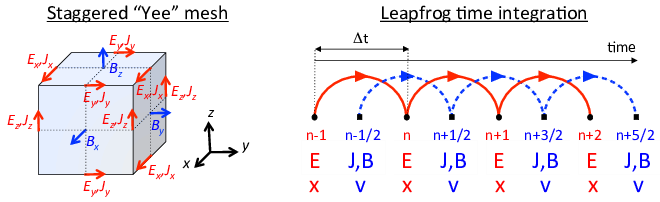
\includegraphics[scale=0.7]{Yee_grid.png}
%\par\end{centering}
\caption{\label{fig:yee_grid}(left) Layout of field components on the staggered ``Yee'' grid. Current densities and electric fields are defined on the edges of the cells and magnetic fields on the faces. (right) Time integration using a second-order finite-difference "leapfrog" integrator.}
\end{figure}

The differential operator is defined as $\nabla=D_{x}\mathbf{\hat{x}}+D_{y}\mathbf{\hat{y}}+D_{z}\mathbf{\hat{z}}$
and the finite-difference operators in time and space are defined
respectively as $ $$D_{t}G|_{i,j,k}^{n}=\left(G|_{i,j,k}^{n+1/2}-G|_{i,j,k}^{n-1/2}\right)/\Delta t$$ $
and $D_{x}G|_{i,j,k}^{n}=\left(G|_{i+1/2,j,k}^{n}-G|_{i-1/2,j,k}^{n}\right)/\Delta x$,
where $\Delta t$ and $\Delta x$ are respectively the time step and
the grid cell size along $x$, $n$ is the time index and $i$, $j$
and $k$ are the spatial indices along $x$, $y$ and $z$ respectively.
The difference operators along $y$ and $z$ are obtained by circular
permutation. The equations in brackets are given for completeness,
as they are often not actually solved, thanks to the usage of a so-called
charge conserving algorithm, as explained below. As shown in Figure
\ref{fig:yee_grid}, the quantities are given on a staggered (or ``Yee'')
grid \cite{Yee}, where the electric field components are located
between nodes and the magnetic field components are located in the
center of the cell faces. Knowing the current densities at half-integer steps, 
the electric field components are updated alternately with the magnetic 
field components at integer and half-integer steps respectively.


%%%%%%%%%%%%%%%%%%%%%%%%%%%%%%%%%%%
\subsubsection{Non-Standard Finite-Difference Time-Domain (NSFDTD)}
%%%%%%%%%%%%%%%%%%%%%%%%%%%%%%%%%%%

\usepackage{bm}
\usepackage{amsmath}
\usepackage{amssymb}
\usepackage{graphicx}
\usepackage{url}
\usepackage{hyperref}

\usepackage[displaymath]{lineno}\usepackage{bm}% bold math

\newcommand{\fe}{\mathbf{\tilde{E}}}
\newcommand{\fb}{\mathbf{\tilde{B}}}
\newcommand{\fj}{\mathbf{\tilde{J}}}
\newcommand{\ff}{\tilde{F}}
\newcommand{\fg}{\tilde{G}}
\newcommand{\fk}{\mathbf{k}}
\newcommand{\fkhat}{\mathbf{\hat{k}}}

% Definitions from Remi's paper on Galilean math
\newcommand{\Km}{\vec{K}_{\vec{m}}}
\newcommand{\km}{\vec{k}_{\vec{m}}}
\renewcommand{\vec}[1]{\boldsymbol{#1}}
\newcommand{\vgal}{\vec{v}_{gal}}
\newcommand{\nab}{\vec{\nabla'}}
\newcommand{\Dt}[1]{ \frac{\partial #1}{\partial t}}
\newcommand{\mc}[1]{\hat{\mathcal{#1}}}
\newcommand{\xj}{\vec{x}'_{\vec{j}}}
\newcommand{\Xll}{\vec{X}_{\vec{\ell}}}
\newcommand{\Integ}[1]{\int_{-\infty}^{\infty} \!\!\!\!\!\!
  \mathrm{d}#1}
\newcommand{\RInteg}[1]{\int_{0}^{\infty} \!\! \frac{#1\mathrm{d}#1}{(2\pi)^2}}

% Definitions from Remi's Thesis
\newcommand{\h}{\mathcal{H}}
\newcommand{\hf}{\frac{1}{2}}
\newcommand{\um}{$\mu$m}
\newcommand{\Um}{\mu \mathrm{m}}
\newcommand{\aal}{\langle \vec{a}_l^2 \rangle}
\newcommand{\etad}{ \eta_d }
\newcommand{\etae}{ \eta_\epsilon }
\newcommand{\etag}{ \eta_\gamma }
\newcommand{\tlambda}{ \tilde{\lambda} }
%\newcommand\comment[1]{\textcolor{red}{\textbf{#1}}}
\newcommand{\gsim}{\mathrel{\hbox{\rlap{\lower.55ex 
\hbox{$\sim$}} \kern-.3em \raise.4ex \hbox{$>$}}}}
\newcommand{\lsim}{\mathrel{\hbox{\rlap{\lower.55ex 
\hbox{$\sim$}} \kern-.3em \raise.4ex \hbox{$<$}}}}
\newcommand{\kfoc}{k_\mathrm{foc}}
\newcommand{\bkfoc}{\bar{k}_\mathrm{foc}}
\newcommand{\xil}{\xi_{\mathrm{laser}}}

\newcommand{\Ex}[2]{{E_x}^{#1}_{#2}}
\newcommand{\Ey}[2]{{E_y}^{#1}_{#2}}
\newcommand{\Ez}[2]{{E_z}^{#1}_{#2}}
\newcommand{\Bx}[2]{{B_x}^{#1}_{#2}}
\newcommand{\By}[2]{{B_y}^{#1}_{#2}}
\newcommand{\Bz}[2]{{B_z}^{#1}_{#2}}
\newcommand{\Jx}[2]{{J_x}^{#1}_{#2}}
\newcommand{\Jy}[2]{{J_y}^{#1}_{#2}}
\newcommand{\Jz}[2]{{J_z}^{#1}_{#2}}

\newcommand{\tEr}[2]{\tilde{E_r}^{#1}_{#2}}
\newcommand{\tEt}[2]{\tilde{E_\theta}^{#1}_{#2}}
\newcommand{\tEz}[2]{\tilde{E_z}^{#1}_{#2}}
\newcommand{\tBr}[2]{\tilde{B_r}^{#1}_{#2}}
\newcommand{\tBt}[2]{\tilde{B_\theta}^{#1}_{#2}}
\newcommand{\tBz}[2]{\tilde{B_z}^{#1}_{#2}}
\newcommand{\tJr}[2]{\tilde{J_r}^{#1}_{#2}}
\newcommand{\tJt}[2]{\tilde{J_\theta}^{#1}_{#2}}
\newcommand{\tJz}[2]{\tilde{J_z}^{#1}_{#2}}

\newcommand{\CCirc}{\textsc{Calder Circ}}
\newcommand{\CCart}{\textsc{Calder 3D}}

In \cite{Coleieee1997,Coleieee2002}, Cole introduced an implementation
of the source-free Maxwell's wave equations for narrow-band applications
based on non-standard finite-differences (NSFD). In \cite{Karkicap06},
Karkkainen \emph{et al.} adapted it for wideband applications. At
the Courant limit for the time step and for a given set of parameters,
the stencil proposed in \cite{Karkicap06} has no numerical dispersion
along the principal axes, provided that the cell size is the same
along each dimension (i.e. cubic cells in 3D). The ``Cole-Karkkainnen''
(or CK) solver uses the non-standard finite difference formulation
(based on extended stencils) of the Maxwell-Ampere equation and can be 
implemented as follows \cite{Vayjcp2011}:

\begin{subequations}
\begin{eqnarray}
D_{t}\mathbf{B} & = & -\nabla^{*}\times\mathbf{E}\label{Eq:Faraday}\\
D_{t}\mathbf{E} & = & \nabla\times\mathbf{B}-\mathbf{J}\label{Eq:Ampere}\\
\left[\nabla\cdot\mathbf{E}\right. & = & \left.\rho\right]\label{Eq:Gauss}\\
\left[\nabla^{*}\cdot\mathbf{B}\right. & = & \left.0\right]\label{Eq:divb}
\end{eqnarray}
\end{subequations}

Eq. \ref{Eq:Gauss} and \ref{Eq:divb} are not being solved explicitly
but verified via appropriate initial conditions and current deposition
procedure. The NSFD differential operators is given by $\nabla^{*}=D_{x}^{*}\mathbf{\hat{x}}+D_{y}^{*}\mathbf{\hat{y}}+D_{z}^{*}\mathbf{\hat{z}}$
where $D_{x}^{*}=\left(\alpha+\beta S_{x}^{1}+\xi S_{x}^{2}\right)D_{x}$
with $S_{x}^{1}G|_{i,j,k}^{n}=G|_{i,j+1,k}^{n}+G|_{i,j-1,k}^{n}+G|_{i,j,k+1}^{n}+G|_{i,j,k-1}^{n}$,
$S_{x}^{2}G|_{i,j,k}^{n}=G|_{i,j+1,k+1}^{n}+G|_{i,j-1,k+1}^{n}+G|_{i,j+1,k-1}^{n}+G|_{i,j-1,k-1}^{n}$.
$G$ is a sample vector component, while $\alpha$, $\beta$ and $\xi$
are constant scalars satisfying $\alpha+4\beta+4\xi=1$. As with
the FDTD algorithm, the quantities with half-integer are located between
the nodes (electric field components) or in the center of the cell
faces (magnetic field components). The operators along $y$ and $z$,
i.e. $D_{y}$, $D_{z}$, $D_{y}^{*}$, $D_{z}^{*}$, $S_{y}^{1}$,
$S_{z}^{1}$, $S_{y}^{2}$, and $S_{z}^{2}$, are obtained by circular
permutation of the indices.

Assuming cubic cells ($\Delta x=\Delta y=\Delta z$), the coefficients
given in \cite{Karkicap06} ($\alpha=7/12$, $\beta=1/12$ and $\xi=1/48$)
allow for the Courant condition to be at $\Delta t=\Delta x$, which
equates to having no numerical dispersion along the principal axes.
The algorithm reduces to the FDTD algorithm with $\alpha=1$ and $\beta=\xi=0$.
An extension to non-cubic cells is provided by Cowan, \emph{et al.}
in 3-D in \cite{CowanPRSTAB13} and was given by Pukhov in 2-D in
\cite{PukhovJPP99}. An alternative NSFDTD implementation that enables superluminous waves is also
given by Lehe {\it et al.} in \cite{LehePRSTAB13}. 

As mentioned above, a key feature of the algorithms based on NSFDTD
is that some implementations \cite{Karkicap06,CowanPRSTAB13} enable the time step $\Delta t=\Delta x$ along one or
more axes and no numerical dispersion along those axes. However, as
shown in \cite{Vayjcp2011}, an instability develops at the Nyquist
wavelength at (or very near) such a timestep. It is also shown in
the same paper that removing the Nyquist component in all the source
terms using a bilinear filter (see description of the filter below)
suppresses this instability.



%%%%%%%%%%%%%%%%%%%%%%%%%%%%%%%%%%%
\subsubsection{Pseudo Spectral Analytical Time Domain (PSATD)}
%%%%%%%%%%%%%%%%%%%%%%%%%%%%%%%%%%%

\usepackage{bm}
\usepackage{amsmath}
\usepackage{amssymb}
\usepackage{graphicx}
\usepackage{url}
\usepackage{hyperref}

\usepackage[displaymath]{lineno}\usepackage{bm}% bold math

\newcommand{\fe}{\mathbf{\tilde{E}}}
\newcommand{\fb}{\mathbf{\tilde{B}}}
\newcommand{\fj}{\mathbf{\tilde{J}}}
\newcommand{\ff}{\tilde{F}}
\newcommand{\fg}{\tilde{G}}
\newcommand{\fk}{\mathbf{k}}
\newcommand{\fkhat}{\mathbf{\hat{k}}}

% Definitions from Remi's paper on Galilean math
\newcommand{\Km}{\vec{K}_{\vec{m}}}
\newcommand{\km}{\vec{k}_{\vec{m}}}
\renewcommand{\vec}[1]{\boldsymbol{#1}}
\newcommand{\vgal}{\vec{v}_{gal}}
\newcommand{\nab}{\vec{\nabla'}}
\newcommand{\Dt}[1]{ \frac{\partial #1}{\partial t}}
\newcommand{\mc}[1]{\hat{\mathcal{#1}}}
\newcommand{\xj}{\vec{x}'_{\vec{j}}}
\newcommand{\Xll}{\vec{X}_{\vec{\ell}}}
\newcommand{\Integ}[1]{\int_{-\infty}^{\infty} \!\!\!\!\!\!
  \mathrm{d}#1}
\newcommand{\RInteg}[1]{\int_{0}^{\infty} \!\! \frac{#1\mathrm{d}#1}{(2\pi)^2}}

% Definitions from Remi's Thesis
\newcommand{\h}{\mathcal{H}}
\newcommand{\hf}{\frac{1}{2}}
\newcommand{\um}{$\mu$m}
\newcommand{\Um}{\mu \mathrm{m}}
\newcommand{\aal}{\langle \vec{a}_l^2 \rangle}
\newcommand{\etad}{ \eta_d }
\newcommand{\etae}{ \eta_\epsilon }
\newcommand{\etag}{ \eta_\gamma }
\newcommand{\tlambda}{ \tilde{\lambda} }
%\newcommand\comment[1]{\textcolor{red}{\textbf{#1}}}
\newcommand{\gsim}{\mathrel{\hbox{\rlap{\lower.55ex 
\hbox{$\sim$}} \kern-.3em \raise.4ex \hbox{$>$}}}}
\newcommand{\lsim}{\mathrel{\hbox{\rlap{\lower.55ex 
\hbox{$\sim$}} \kern-.3em \raise.4ex \hbox{$<$}}}}
\newcommand{\kfoc}{k_\mathrm{foc}}
\newcommand{\bkfoc}{\bar{k}_\mathrm{foc}}
\newcommand{\xil}{\xi_{\mathrm{laser}}}

\newcommand{\Ex}[2]{{E_x}^{#1}_{#2}}
\newcommand{\Ey}[2]{{E_y}^{#1}_{#2}}
\newcommand{\Ez}[2]{{E_z}^{#1}_{#2}}
\newcommand{\Bx}[2]{{B_x}^{#1}_{#2}}
\newcommand{\By}[2]{{B_y}^{#1}_{#2}}
\newcommand{\Bz}[2]{{B_z}^{#1}_{#2}}
\newcommand{\Jx}[2]{{J_x}^{#1}_{#2}}
\newcommand{\Jy}[2]{{J_y}^{#1}_{#2}}
\newcommand{\Jz}[2]{{J_z}^{#1}_{#2}}

\newcommand{\tEr}[2]{\tilde{E_r}^{#1}_{#2}}
\newcommand{\tEt}[2]{\tilde{E_\theta}^{#1}_{#2}}
\newcommand{\tEz}[2]{\tilde{E_z}^{#1}_{#2}}
\newcommand{\tBr}[2]{\tilde{B_r}^{#1}_{#2}}
\newcommand{\tBt}[2]{\tilde{B_\theta}^{#1}_{#2}}
\newcommand{\tBz}[2]{\tilde{B_z}^{#1}_{#2}}
\newcommand{\tJr}[2]{\tilde{J_r}^{#1}_{#2}}
\newcommand{\tJt}[2]{\tilde{J_\theta}^{#1}_{#2}}
\newcommand{\tJz}[2]{\tilde{J_z}^{#1}_{#2}}

\newcommand{\CCirc}{\textsc{Calder Circ}}
\newcommand{\CCart}{\textsc{Calder 3D}}

Maxwell's equations in Fourier space are given by % --- Maxwell
\begin{subequations}
\begin{eqnarray}
\frac{\partial\fe}{\partial t} & = & c^2i\fk\times\fb-\frac{1}{\epsilon_0} \fj\\
\frac{\partial\fb}{\partial t} & = & -i\fk\times\fe\\
{}[i\fk\cdot\fe & = & \frac{\tilde{\rho}}{\epsilon_0}]\\
{}[i\fk\cdot\fb & = & 0]
\end{eqnarray}
\end{subequations}
where $\tilde{a}$ is the Fourier Transform of the quantity $a$.
As with the real space formulation, provided that the continuity equation
$\partial\tilde{\rho}/\partial t+i\fk\cdot\fj=0$ is satisfied, then
the last two equations will automatically be satisfied at any time
if satisfied initially and do not need to be explicitly integrated.

These equations can be integrated analytically over one timestep,
assuming that the current density $\fj$ is constant over this timestep, and that
the charge density is linear in time ($\tilde{\rho}(t) = \tilde{\rho}^n +
\frac{\tilde{\rho}^{n+1}-\tilde{\rho}^n}{\Delta t}(t-n\Delta t)$). This gives:
\begin{subequations}
\begin{eqnarray}
\fe^{n+1} & = & C\fe^{n}+\frac{S}{ck}\left(c^2i\fk\times\fb^{n}-\frac{1}{\epsilon_0}\fj^{n+1/2}\right) \\
 & - & i\fk\left[ \frac{1}{\epsilon_0 k^2}\left( 1 - \frac{S}{ck\Delta t} \right)\tilde{\rho}^{n+1}
 - \frac{1}{\epsilon_0 k^2}\left( C - \frac{S}{ck\Delta t} \right)\tilde{\rho}^{n}\right]\nonumber \\
 fb^{n+1} & = & C\fb^{n}-\frac{S}{ck}i\fk\times\fe^{n}\\
&+&\frac{1}{\epsilon_0}\frac{1-C}{c^2k^2}i\fk\times\fj^{n+1/2}.\label{Eq_PSATD_2}
\end{eqnarray}
\end{subequations}
with $C=\cos\left(c k\Delta t\right)$ and $S=\sin\left(c k\Delta t\right)$.

For fields generated by the source terms without the self-consistent
dynamics of the charged particles, this algorithm is free of numerical
dispersion and is not subject to a Courant condition. Furthermore,
this solution is exact for any time step size subject to the assumption
that the current source is constant over that time step.

As shown in \cite{VayJCP13}, by expanding the coefficients $S_{h}$
and $C_{h}$ in Taylor series and keeping the leading terms, the PSATD
formulation reduces to the perhaps better known pseudo-spectral time-domain
(PSTD) formulation \cite{DawsonRMP83,Liumotl1997}: % --- PSTD
\begin{subequations}
\begin{eqnarray}
\fe^{n+1} & = & \fe^{n}+ic^2\Delta t\fk\times\fb^{n+1/2}-\frac{\Delta t}{\epsilon_0}\fj^{n+1/2},\\
\fb^{n+3/2} & = & \fb^{n+1/2}-i\Delta t\fk\times\fe^{n+1}.
\end{eqnarray}
\end{subequations}
The dispersion relation of the PSTD solver is given by $\sin(\frac{\omega\Delta t}{2})=\frac{k\Delta t}{2}.$
In contrast to the PSATD solver, the PSTD solver is subject to numerical
dispersion for a finite time step and to a Courant condition that
is given by $\Delta t\leq \frac{2}{\pi}\left(\frac{1}{\Delta x^{2}}+\frac{1}{\Delta y^{2}}+\frac{1}{\Delta x^{2}}\right)^{-1/2}.$

The PSATD and PSTD formulations that were just given apply to the
field components located at the nodes of the grid. As noted in \cite{Ohmurapiers2010},
they can also be easily recast on a staggered Yee grid by multiplication
of the field components by the appropriate phase factors to shift
them from the collocated to the staggered locations. The choice between
a collocated and a staggered formulation is application-dependent.

Spectral solvers used to be very popular in the years 1970s to early 1990s, before being replaced by finite-difference methods with the advent of parallel supercomputers that favored local methods. However, it was shown recently that standard domain decomposition with Fast Fourier Transforms that are local to each subdomain could be used effectively with PIC spectral methods \cite{VayJCP13}, at the cost of truncation errors in the guard cells that could be neglected. A detailed analysis of the effectiveness of the method with exact evaluation of the magnitude of the effect of the truncation error is given in \cite{Vincenti2016a} for stencils of arbitrary order (up-to the infinite ``spectral'' order).


%%%%%%%%%%%%%%%%%%%%%%%%%%%%%%%%%%%
\subsection{Current deposition}
%%%%%%%%%%%%%%%%%%%%%%%%%%%%%%%%%%%

\usepackage{bm}
\usepackage{amsmath}
\usepackage{amssymb}
\usepackage{graphicx}
\usepackage{url}
\usepackage{hyperref}

\usepackage[displaymath]{lineno}\usepackage{bm}% bold math

\newcommand{\fe}{\mathbf{\tilde{E}}}
\newcommand{\fb}{\mathbf{\tilde{B}}}
\newcommand{\fj}{\mathbf{\tilde{J}}}
\newcommand{\ff}{\tilde{F}}
\newcommand{\fg}{\tilde{G}}
\newcommand{\fk}{\mathbf{k}}
\newcommand{\fkhat}{\mathbf{\hat{k}}}

% Definitions from Remi's paper on Galilean math
\newcommand{\Km}{\vec{K}_{\vec{m}}}
\newcommand{\km}{\vec{k}_{\vec{m}}}
\renewcommand{\vec}[1]{\boldsymbol{#1}}
\newcommand{\vgal}{\vec{v}_{gal}}
\newcommand{\nab}{\vec{\nabla'}}
\newcommand{\Dt}[1]{ \frac{\partial #1}{\partial t}}
\newcommand{\mc}[1]{\hat{\mathcal{#1}}}
\newcommand{\xj}{\vec{x}'_{\vec{j}}}
\newcommand{\Xll}{\vec{X}_{\vec{\ell}}}
\newcommand{\Integ}[1]{\int_{-\infty}^{\infty} \!\!\!\!\!\!
  \mathrm{d}#1}
\newcommand{\RInteg}[1]{\int_{0}^{\infty} \!\! \frac{#1\mathrm{d}#1}{(2\pi)^2}}

% Definitions from Remi's Thesis
\newcommand{\h}{\mathcal{H}}
\newcommand{\hf}{\frac{1}{2}}
\newcommand{\um}{$\mu$m}
\newcommand{\Um}{\mu \mathrm{m}}
\newcommand{\aal}{\langle \vec{a}_l^2 \rangle}
\newcommand{\etad}{ \eta_d }
\newcommand{\etae}{ \eta_\epsilon }
\newcommand{\etag}{ \eta_\gamma }
\newcommand{\tlambda}{ \tilde{\lambda} }
%\newcommand\comment[1]{\textcolor{red}{\textbf{#1}}}
\newcommand{\gsim}{\mathrel{\hbox{\rlap{\lower.55ex 
\hbox{$\sim$}} \kern-.3em \raise.4ex \hbox{$>$}}}}
\newcommand{\lsim}{\mathrel{\hbox{\rlap{\lower.55ex 
\hbox{$\sim$}} \kern-.3em \raise.4ex \hbox{$<$}}}}
\newcommand{\kfoc}{k_\mathrm{foc}}
\newcommand{\bkfoc}{\bar{k}_\mathrm{foc}}
\newcommand{\xil}{\xi_{\mathrm{laser}}}

\newcommand{\Ex}[2]{{E_x}^{#1}_{#2}}
\newcommand{\Ey}[2]{{E_y}^{#1}_{#2}}
\newcommand{\Ez}[2]{{E_z}^{#1}_{#2}}
\newcommand{\Bx}[2]{{B_x}^{#1}_{#2}}
\newcommand{\By}[2]{{B_y}^{#1}_{#2}}
\newcommand{\Bz}[2]{{B_z}^{#1}_{#2}}
\newcommand{\Jx}[2]{{J_x}^{#1}_{#2}}
\newcommand{\Jy}[2]{{J_y}^{#1}_{#2}}
\newcommand{\Jz}[2]{{J_z}^{#1}_{#2}}

\newcommand{\tEr}[2]{\tilde{E_r}^{#1}_{#2}}
\newcommand{\tEt}[2]{\tilde{E_\theta}^{#1}_{#2}}
\newcommand{\tEz}[2]{\tilde{E_z}^{#1}_{#2}}
\newcommand{\tBr}[2]{\tilde{B_r}^{#1}_{#2}}
\newcommand{\tBt}[2]{\tilde{B_\theta}^{#1}_{#2}}
\newcommand{\tBz}[2]{\tilde{B_z}^{#1}_{#2}}
\newcommand{\tJr}[2]{\tilde{J_r}^{#1}_{#2}}
\newcommand{\tJt}[2]{\tilde{J_\theta}^{#1}_{#2}}
\newcommand{\tJz}[2]{\tilde{J_z}^{#1}_{#2}}

\newcommand{\CCirc}{\textsc{Calder Circ}}
\newcommand{\CCart}{\textsc{Calder 3D}}

The current densities are deposited on the computational grid from
the particle position and velocities, employing splines of various
orders \cite{Abejcp86}.

\begin{subequations}
\begin{eqnarray}
\rho & = & \frac{1}{\Delta x \Delta y \Delta z}\sum_nq_nS_n\\
\mathbf{J} & = & \frac{1}{\Delta x \Delta y \Delta z}\sum_nq_n\mathbf{v_n}S_n
\end{eqnarray}
\end{subequations}

In most applications, it is essential to prevent the accumulation
of errors resulting from the violation of the discretized Gauss' Law.
This is accomplished by providing a method for depositing the current
from the particles to the grid that preserves the discretized Gauss'
Law, or by providing a mechanism for ``divergence cleaning'' \cite{Birdsalllangdon,Langdoncpc92,Marderjcp87,Vaypop98,Munzjcp2000}.
For the former, schemes that allow a deposition of the current that
is exact when combined with the Yee solver is given in \cite{Villasenorcpc92}
for linear splines and in \cite{Esirkepovcpc01} for splines of arbitrary order. 

The NSFDTD formulations given above and in \cite{PukhovJPP99,Vayjcp2011,CowanPRSTAB13,LehePRSTAB13} 
apply to the Maxwell-Faraday
equation, while the discretized Maxwell-Ampere equation uses the FDTD
formulation. Consequently, the charge conserving algorithms developed
for current deposition \cite{Villasenorcpc92,Esirkepovcpc01} apply
readily to those NSFDTD-based formulations. More details concerning
those implementations, including the expressions for the numerical
dispersion and Courant condition are given 
in \cite{PukhovJPP99,Vayjcp2011,CowanPRSTAB13,LehePRSTAB13}. 

In the case of the pseudospectral solvers, the current deposition
algorithm generally does not satisfy the discretized continuity equation
in Fourier space $\tilde{\rho}^{n+1}=\tilde{\rho}^{n}-i\Delta t\fk\cdot\mathbf{\tilde{J}}^{n+1/2}$.
In this case, a Boris correction \cite{Birdsalllangdon} can be applied
in $k$ space in the form $\fe_{c}^{n+1}=\fe^{n+1}-\left(\fk\cdot\fe^{n+1}+i\tilde{\rho}^{n+1}\right)\fkhat/k$,
where $\fe_{c}$ is the corrected field. Alternatively, a correction
to the current can be applied (with some similarity to the current
deposition presented by Morse and Nielson in their potential-based
model in \cite{Morsenielson1971}) using $\fj_{c}^{n+1/2}=\fj^{n+1/2}-\left[\fk\cdot\fj^{n+1/2}-i\left(\tilde{\rho}^{n+1}-\tilde{\rho}^{n}\right)/\Delta t\right]\fkhat/k$,
where $\fj_{c}$ is the corrected current. In this case, the transverse
component of the current is left untouched while the longitudinal
component is effectively replaced by the one obtained from integration
of the continuity equation, ensuring that the corrected current satisfies
the continuity equation. The advantage of correcting the current rather than 
the electric field is that it is more local and thus more compatible with 
domain decomposition of the fields for parallel computation \cite{VayJCP2013}.

Alternatively, an exact current deposition can be written for the pseudospectral solvers, following the geometrical interpretation of existing methods in real space \cite{Morsenielson1971,Villasenorcpc92,Esirkepovcpc01}, thereby averaging the currents of the paths following grid lines between positions $(x^n,y^n)$ and $(x^{n+1},y^{n+1})$, which is given in 2D (extension to 3D follows readily) for $k\neq0$ by  \cite{VayJCP2013}:
%
\begin{eqnarray}
\fj^{k\neq0}=\frac{i\mathbf{\tilde{D}}}{\fk}
\end{eqnarray}
with 
\begin{eqnarray}
D_x   =  \frac{1}{2\Delta t}\sum_i q_i
  [\Gamma(x_i^{n+1},y_i^{n+1})-\Gamma(x_i^{n},y_i^{n+1}) \nonumber\\ 
+\Gamma(x_i^{n+1},y_i^{n})-\Gamma(x_i^{n},y_i^{n})],\\
D_y   =  \frac{1}{2\Delta t}\sum_i q_i
  [\Gamma(x_i^{n+1},y_i^{n+1})-\Gamma(x_i^{n+1},y_i^{n}) \nonumber \\
+\Gamma(x_i^{n},y_i^{n+1})-\Gamma(x_i^{n},y_i^{n})],
\end{eqnarray}
where $\Gamma$ is the macro-particle form factor. 
%
The contributions for $k=0$ are integrated directly in real space  \cite{VayJCP2013}.


%%%%%%%%%%%%%%%%%%%%%%%%%%%%%%%%%%%
\subsection{Field gather}
%%%%%%%%%%%%%%%%%%%%%%%%%%%%%%%%%%%

\usepackage{bm}
\usepackage{amsmath}
\usepackage{amssymb}
\usepackage{graphicx}
\usepackage{url}
\usepackage{hyperref}

\usepackage[displaymath]{lineno}\usepackage{bm}% bold math

\newcommand{\fe}{\mathbf{\tilde{E}}}
\newcommand{\fb}{\mathbf{\tilde{B}}}
\newcommand{\fj}{\mathbf{\tilde{J}}}
\newcommand{\ff}{\tilde{F}}
\newcommand{\fg}{\tilde{G}}
\newcommand{\fk}{\mathbf{k}}
\newcommand{\fkhat}{\mathbf{\hat{k}}}

% Definitions from Remi's paper on Galilean math
\newcommand{\Km}{\vec{K}_{\vec{m}}}
\newcommand{\km}{\vec{k}_{\vec{m}}}
\renewcommand{\vec}[1]{\boldsymbol{#1}}
\newcommand{\vgal}{\vec{v}_{gal}}
\newcommand{\nab}{\vec{\nabla'}}
\newcommand{\Dt}[1]{ \frac{\partial #1}{\partial t}}
\newcommand{\mc}[1]{\hat{\mathcal{#1}}}
\newcommand{\xj}{\vec{x}'_{\vec{j}}}
\newcommand{\Xll}{\vec{X}_{\vec{\ell}}}
\newcommand{\Integ}[1]{\int_{-\infty}^{\infty} \!\!\!\!\!\!
  \mathrm{d}#1}
\newcommand{\RInteg}[1]{\int_{0}^{\infty} \!\! \frac{#1\mathrm{d}#1}{(2\pi)^2}}

% Definitions from Remi's Thesis
\newcommand{\h}{\mathcal{H}}
\newcommand{\hf}{\frac{1}{2}}
\newcommand{\um}{$\mu$m}
\newcommand{\Um}{\mu \mathrm{m}}
\newcommand{\aal}{\langle \vec{a}_l^2 \rangle}
\newcommand{\etad}{ \eta_d }
\newcommand{\etae}{ \eta_\epsilon }
\newcommand{\etag}{ \eta_\gamma }
\newcommand{\tlambda}{ \tilde{\lambda} }
%\newcommand\comment[1]{\textcolor{red}{\textbf{#1}}}
\newcommand{\gsim}{\mathrel{\hbox{\rlap{\lower.55ex 
\hbox{$\sim$}} \kern-.3em \raise.4ex \hbox{$>$}}}}
\newcommand{\lsim}{\mathrel{\hbox{\rlap{\lower.55ex 
\hbox{$\sim$}} \kern-.3em \raise.4ex \hbox{$<$}}}}
\newcommand{\kfoc}{k_\mathrm{foc}}
\newcommand{\bkfoc}{\bar{k}_\mathrm{foc}}
\newcommand{\xil}{\xi_{\mathrm{laser}}}

\newcommand{\Ex}[2]{{E_x}^{#1}_{#2}}
\newcommand{\Ey}[2]{{E_y}^{#1}_{#2}}
\newcommand{\Ez}[2]{{E_z}^{#1}_{#2}}
\newcommand{\Bx}[2]{{B_x}^{#1}_{#2}}
\newcommand{\By}[2]{{B_y}^{#1}_{#2}}
\newcommand{\Bz}[2]{{B_z}^{#1}_{#2}}
\newcommand{\Jx}[2]{{J_x}^{#1}_{#2}}
\newcommand{\Jy}[2]{{J_y}^{#1}_{#2}}
\newcommand{\Jz}[2]{{J_z}^{#1}_{#2}}

\newcommand{\tEr}[2]{\tilde{E_r}^{#1}_{#2}}
\newcommand{\tEt}[2]{\tilde{E_\theta}^{#1}_{#2}}
\newcommand{\tEz}[2]{\tilde{E_z}^{#1}_{#2}}
\newcommand{\tBr}[2]{\tilde{B_r}^{#1}_{#2}}
\newcommand{\tBt}[2]{\tilde{B_\theta}^{#1}_{#2}}
\newcommand{\tBz}[2]{\tilde{B_z}^{#1}_{#2}}
\newcommand{\tJr}[2]{\tilde{J_r}^{#1}_{#2}}
\newcommand{\tJt}[2]{\tilde{J_\theta}^{#1}_{#2}}
\newcommand{\tJz}[2]{\tilde{J_z}^{#1}_{#2}}

\newcommand{\CCirc}{\textsc{Calder Circ}}
\newcommand{\CCart}{\textsc{Calder 3D}}

In general, the field is gathered from the mesh onto the macroparticles
using splines of the same order as for the current deposition $\mathbf{S}=\left(S_{x},S_{y},S_{z}\right)$.
Three variations are considered:
\begin{itemize}
\item ``momentum conserving'': fields are interpolated from the grid nodes
to the macroparticles using $\mathbf{S}=\left(S_{nx},S_{ny},S_{nz}\right)$
for all field components (if the fields are known at staggered positions,
they are first interpolated to the nodes on an auxiliary grid),
\item ``energy conserving (or Galerkin)'': fields are interpolated from
the staggered Yee grid to the macroparticles using $\left(S_{nx-1},S_{ny},S_{nz}\right)$
for $E_{x}$, $\left(S_{nx},S_{ny-1},S_{nz}\right)$ for $E_{y}$,
$\left(S_{nx},S_{ny},S_{nz-1}\right)$ for $E_{z}$, $\left(S_{nx},S_{ny-1},S_{nz-1}\right)$
for $B_{x}$, $\left(S_{nx-1},S_{ny},S_{nz-1}\right)$ for $B{}_{y}$
and$\left(S_{nx-1},S_{ny-1},S_{nz}\right)$ for $B_{z}$ (if the fields
are known at the nodes, they are first interpolated to the staggered
positions on an auxiliary grid),
\item ``uniform'': fields are interpolated directly form the Yee grid
to the macroparticles using $\mathbf{S}=\left(S_{nx},S_{ny},S_{nz}\right)$
for all field components (if the fields are known at the nodes, they
are first interpolated to the staggered positions on an auxiliary
grid).
\end{itemize}
As shown in \cite{BirdsallLangdon,HockneyEastwoodBook,LewisJCP1972},
the momentum and energy conserving schemes conserve momentum and energy
respectively at the limit of infinitesimal time steps and generally
offer better conservation of the respective quantities for a finite
time step. The uniform scheme does not conserve momentum nor energy
in the sense defined for the others but is given for completeness,
as it has been shown to offer some interesting properties in the modeling
of relativistically drifting plasmas \cite{GodfreyJCP2013}.


%%%%%%%%%%%%%%%%%%%%%%%%%%%%%%%%%%%
\section{Filtering}
%%%%%%%%%%%%%%%%%%%%%%%%%%%%%%%%%%%

It is common practice to apply digital filtering to the charge or
current density in Particle-In-Cell simulations as a complement or
an alternative to using higher order splines \cite{Birdsalllangdon}.
A commonly used filter in PIC simulations is the three points filter
$\phi_{j}^{f}=\alpha\phi_{j}+\left(1-\alpha\right)\left(\phi_{j-1}+\phi_{j+1}\right)/2$
where $\phi^{f}$ is the filtered quantity. This filter is called
a bilinear filter when $\alpha=0.5$. Assuming $\phi=e^{jkx}$ and
$\phi^{f}=g\left(\alpha,k\right)e^{jkx}$, the filter gain $g$ is
given as a function of the filtering coefficient $\alpha$ and
the wavenumber $k$ by $g\left(\alpha,k\right)=\alpha+\left(1-\alpha\right)\cos\left(k\Delta x\right)\approx1-\left(1-\alpha\right)\frac{\left(k\Delta x\right)^{2}}{2}+O\left(k^{4}\right)$.
The total attenuation $G$ for $n$ successive applications of filters
of coefficients $\alpha_{1}$...$\alpha_{n}$ is given by $G=\prod_{i=1}^{n}g\left(\alpha_{i},k\right)\approx1-\left(n-\sum_{i=1}^{n}\alpha_{i}\right)\frac{\left(k\Delta x\right)^{2}}{2}+O\left(k^{4}\right)$.
A sharper cutoff in $k$ space is provided by using $\alpha_{n}=n-\sum_{i=1}^{n-1}\alpha_{i}$,
so that $G\approx1+O\left(k^{4}\right)$. Such step is called a ``compensation''
step \cite{Birdsalllangdon}. For the bilinear filter ($\alpha=1/2$),
the compensation factor is $\alpha_{c}=2-1/2=3/2$. For a succession
of $n$ applications of the bilinear factor, it is $\alpha_{c}=n/2+1$.

It is sometimes necessary to filter on a relatively wide band of wavelength,
necessitating the application of a large number of passes of the bilinear
filter or on the use of filters acting on many points. The former
can become very intensive computationally while the latter is problematic
for parallel computations using domain decomposition, as the footprint
of the filter may eventually surpass the size of subdomains. A workaround
is to use a combination of filters of limited footprint. A solution
based on the combination of three point filters with various strides
was proposed in \cite{Vayjcp2011} and operates as follows.

The bilinear filter provides complete suppression of the signal at
the grid Nyquist wavelength (twice the grid cell size). Suppression
of the signal at integer multiples of the Nyquist wavelength can be
obtained by using a stride $s$ in the filter $\phi_{j}^{f}=\alpha\phi_{j}+\left(1-\alpha\right)\left(\phi_{j-s}+\phi_{j+s}\right)/2$
for which the gain is given by $g\left(\alpha,k\right)=\alpha+\left(1-\alpha\right)\cos\left(sk\Delta x\right)\approx1-\left(1-\alpha\right)\frac{\left(sk\Delta x\right)^{2}}{2}+O\left(k^{4}\right)$.
For a given stride, the gain is given by the gain of the bilinear
filter shifted in k space, with the pole $g=0$ shifted from the wavelength
$\lambda=2/\Delta x$ to $\lambda=2s/\Delta x$, with additional poles,
as given by $sk\Delta x=\arccos\left(\frac{\alpha}{\alpha-1}\right)\pmod{2\pi}$.
The resulting filter is pass band between the poles, but since the
poles are spread at different integer values in k space, a wide band
low pass filter can be constructed by combining filters using different
strides. As shown in \cite{Vayjcp2011}, the successive application
of 4-passes + compensation of filters with strides 1, 2 and 4 has
a nearly equivalent fall-off in gain as 80 passes + compensation of
a bilinear filter. Yet, the strided filter solution needs only 15
passes of a three-point filter, compared to 81 passes for an equivalent
n-pass bilinear filter, yielding a gain of 5.4 in number of operations
in favor of the combination of filters with stride. The width of the
filter with stride 4 extends only on 9 points, compared to 81 points
for a single pass equivalent filter, hence giving a gain of 9 in compactness
for the stride filters combination in comparison to the single-pass
filter with large stencil, resulting in more favorable scaling with the number
of computational cores for parallel calculations.

%%%%%%%%%%%%%%%%%%%%%%%%%%%%%%%%%%
%\section{Porting onto new architectures, parallelization, vectorization, mesh refinement}
%%%%%%%%%%%%%%%%%%%%%%%%%%%%%%%%%%


%%%%%%%%%%%%%%%%%%%%%%%%%%%%%%%%%%%%%%%%%%%
%% Just a reminder that you may have to run bibtex
%% All of it up to \end{document} can be removed
%% if you don't like the warning.
%%%%%%%%%%%%%%%%%%%%%%%%%%%%%%%%%%%%%%%%%%%
\IfFileExists{\jobname.bbl}{} {\typeout{} \typeout{{*}{*}{*}{*}{*}{*}{*}{*}{*}{*}{*}{*}{*}{*}{*}{*}{*}{*}{*}{*}{*}{*}{*}{*}{*}{*}{*}{*}{*}{*}{*}{*}{*}{*}{*}{*}{*}{*}{*}{*}{*}{*}}
\typeout{{*}{*} Please run \textquotedbl{}bibtex \jobname\textquotedbl{}
to optain} \typeout{{*}{*} the bibliography and then re-run LaTeX}
\typeout{{*}{*} twice to fix the references!} \typeout{{*}{*}{*}{*}{*}{*}{*}{*}{*}{*}{*}{*}{*}{*}{*}{*}{*}{*}{*}{*}{*}{*}{*}{*}{*}{*}{*}{*}{*}{*}{*}{*}{*}{*}{*}{*}{*}{*}{*}{*}{*}{*}}
\typeout{} }



\end{document}
